\section{Result}
\subsection{Part 1}
In the first part the peak which was measured from the white diode was located at \SI{454.17}{\nano\m}. Using the data obtained from the measurements \autoref{fig:part1} was obtained. From the linear fit in \autoref{fig:a} one can see that that the linear fit intersects the x-axis at $V_\text{in}=\SI{2.7}{\V}$. This means that a voltage under this value would yield no current output, which can be seen in the figure. Thus, one can conclude that the forward bias is $V_\text{in}=\SI{2.7}{\V}$. 

\begin{figure}[H]
    \centering
    \subfloat[This plot displays the itensity of the LED over the current in the circuit. ]{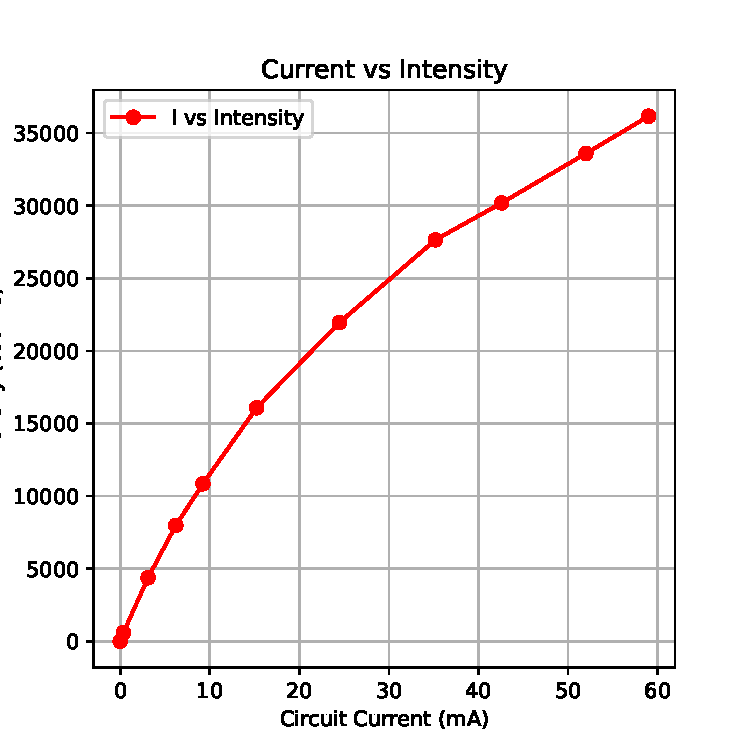
\includegraphics[width=0.49\textwidth]{Figures/part1(b).pdf} \label{fig:a}}
    \hfill
    \subfloat[This plot displays the itensity of the LED over the voltage across the LED in the circuit.]{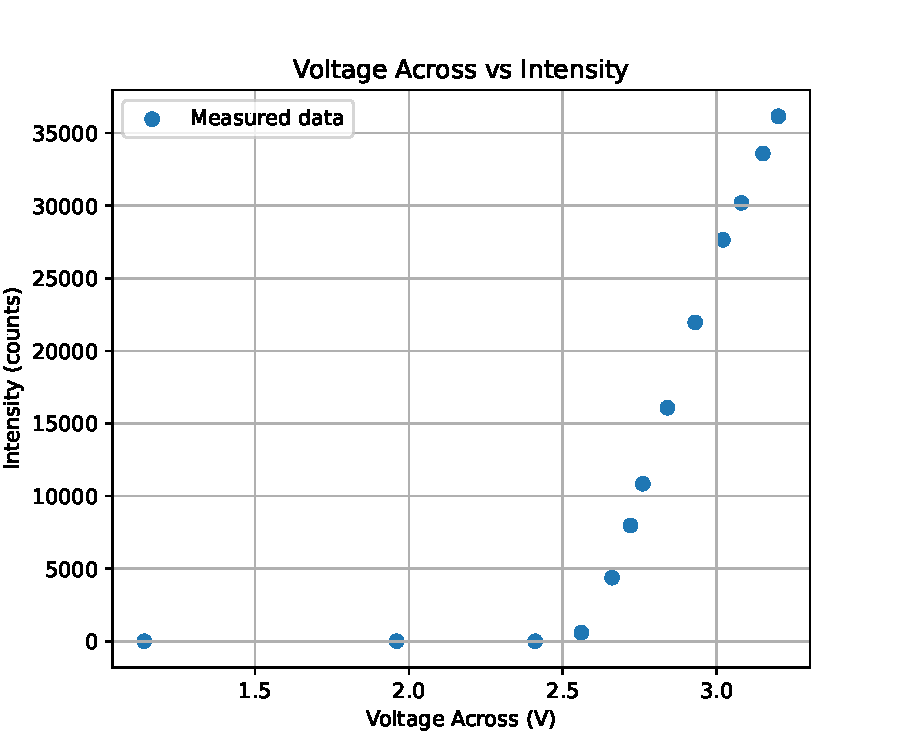
\includegraphics[width=0.49\textwidth]{Figures/part1(c).pdf} \label{fig:b}}
    
    \vspace{0.5cm}
    
    \subfloat[This plot displays the current in the circuit over the voltage from DC-source. A linear fit was used for the non-zero measurements, since this fit would be used to calculate the forward bias. ]{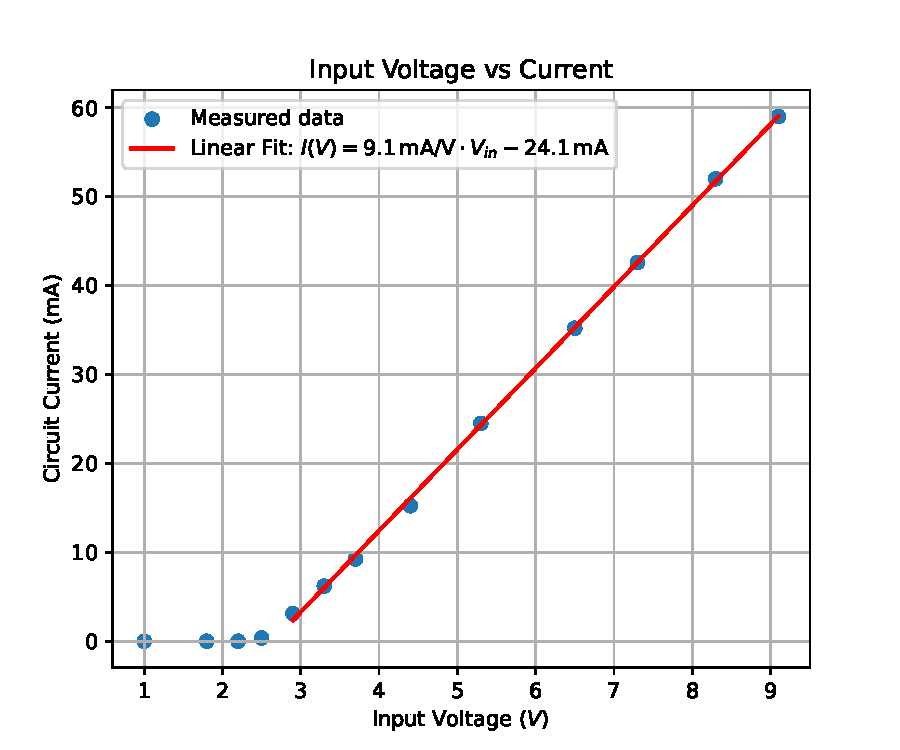
\includegraphics[width=0.49\textwidth]{Figures/part1(a).pdf} \label{fig:c}}

    \caption{Plots of the measurements.}
    \label{fig:part1}
\end{figure}




\subsection{Part 2}
The measurements from the circuit before was combined with the measurements from the program, as seen in \autoref{fig:part2}, in \autoref{tab:part2}. Notably the wavelength of the peak shifted, and the intensity increased when the diode was submerged in liquid nitrogen.

\begin{table}[H]
    \centering
    \caption{This table shows the measurements.}
    \begin{tabular}{@{}llllll@{}}
    \toprule
    Measurement      & V\textsubscript{in} (V) & V\textsubscript{LED} (V) & I\textsubscript{circuit} (mA) & $\lambda_\text{peak}$ (nm) & Intensity (counts) \\ \midrule
    Room temperature & 5.0& 2.06& 30.8& 596.70& 2663.70\\
    Liquid nitrogen  & 5.0& 4.44                     & 7.7& 569.69& 10757.70\\ \bottomrule
    \end{tabular}
    \label{tab:part2}
    \end{table}


\begin{figure}[H]
    \centering
    \subfloat[This was the output from the program at room temperature.]{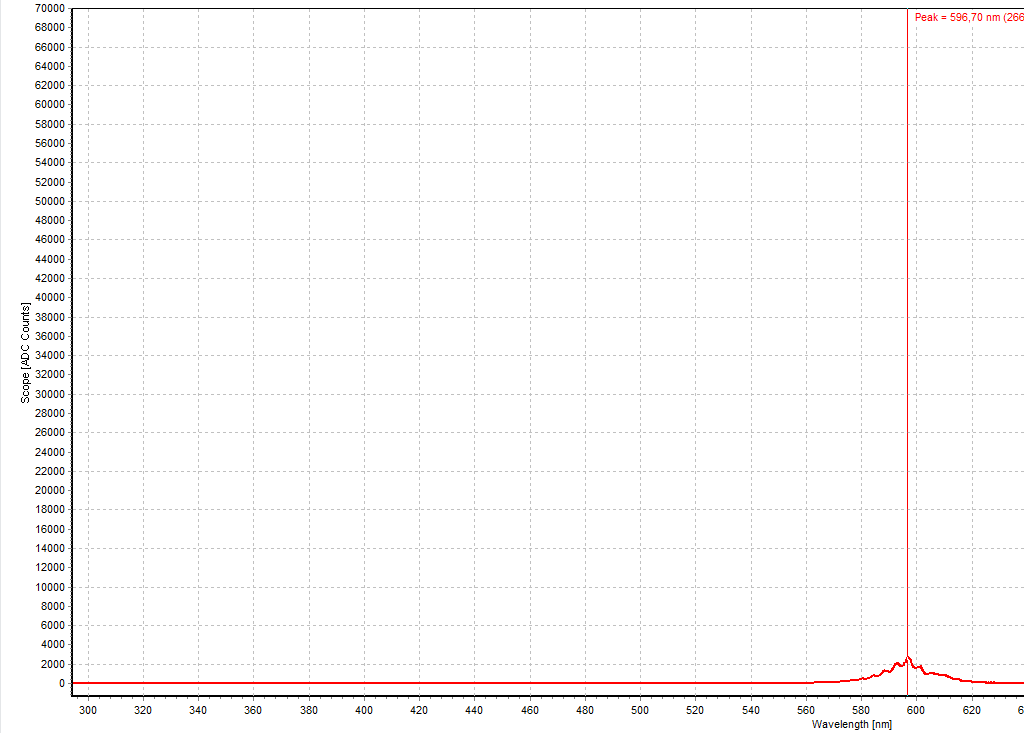
\includegraphics[width=0.39\textwidth]{Figures/Part2_before2.png} \label{fig:before}}
    \hfill
    \subfloat[This was the output from the program when submerged in liquid nitrogen.]{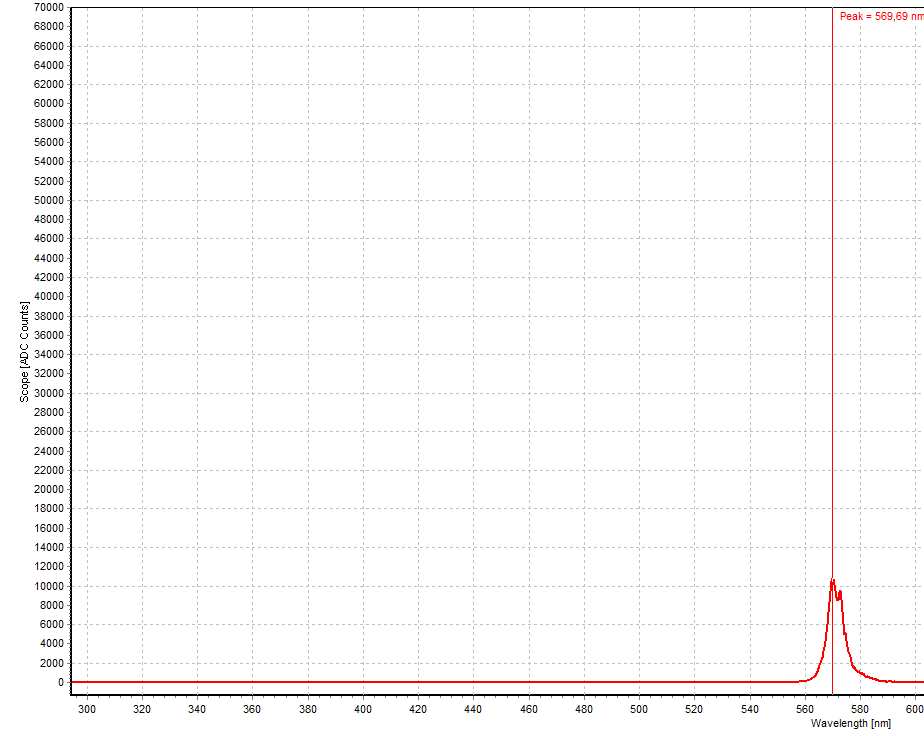
\includegraphics[width=0.39\textwidth]{Figures/Part2_after2.png} \label{fig:after}}
    \caption{This figure display the output from AvaSoft at the different measurements.}
    \label{fig:part2}
\end{figure}




\subsection{Part 3}
The result from the different diode constellations as detectors and emitters can be seen in \autoref{tab:part3}. The table shows that shorter wavelength diodes can excite longer wavelength diodes, but not the other way around.

\begin{table}[H]
    \centering
    \caption{This table displays which combinations of detectors and emitters yielded an voltage output from the diode in the smaller circuit.}
    \begin{tabular}{@{}llll@{}}
    \toprule
    Emitter | Detector: & Red    & Green     & Blue      \\ \midrule
    Red              & Output & No output & No output \\
    Green            & Output & Output    & No output \\
    Blue             & Output & Output    & Output    \\ \bottomrule
    \end{tabular}
    \label{tab:part3}
\end{table}